% Options for packages loaded elsewhere
\PassOptionsToPackage{unicode}{hyperref}
\PassOptionsToPackage{hyphens}{url}
\PassOptionsToPackage{dvipsnames,svgnames*,x11names*}{xcolor}
%
\documentclass[
]{article}
\usepackage{amsmath,amssymb}
\usepackage{lmodern}
\usepackage{ifxetex,ifluatex}
\ifnum 0\ifxetex 1\fi\ifluatex 1\fi=0 % if pdftex
  \usepackage[T1]{fontenc}
  \usepackage[utf8]{inputenc}
  \usepackage{textcomp} % provide euro and other symbols
\else % if luatex or xetex
  \usepackage{unicode-math}
  \defaultfontfeatures{Scale=MatchLowercase}
  \defaultfontfeatures[\rmfamily]{Ligatures=TeX,Scale=1}
\fi
% Use upquote if available, for straight quotes in verbatim environments
\IfFileExists{upquote.sty}{\usepackage{upquote}}{}
\IfFileExists{microtype.sty}{% use microtype if available
  \usepackage[]{microtype}
  \UseMicrotypeSet[protrusion]{basicmath} % disable protrusion for tt fonts
}{}
\makeatletter
\@ifundefined{KOMAClassName}{% if non-KOMA class
  \IfFileExists{parskip.sty}{%
    \usepackage{parskip}
  }{% else
    \setlength{\parindent}{0pt}
    \setlength{\parskip}{6pt plus 2pt minus 1pt}}
}{% if KOMA class
  \KOMAoptions{parskip=half}}
\makeatother
\usepackage{xcolor}
\IfFileExists{xurl.sty}{\usepackage{xurl}}{} % add URL line breaks if available
\IfFileExists{bookmark.sty}{\usepackage{bookmark}}{\usepackage{hyperref}}
\hypersetup{
  pdftitle={Technical comment on `Negative-assortative mating for color in wolves'},
  colorlinks=true,
  linkcolor=blue,
  filecolor=Maroon,
  citecolor=Blue,
  urlcolor=Blue,
  pdfcreator={LaTeX via pandoc}}
\urlstyle{same} % disable monospaced font for URLs
\usepackage[margin=1in]{geometry}
\usepackage{longtable,booktabs,array}
\usepackage{calc} % for calculating minipage widths
% Correct order of tables after \paragraph or \subparagraph
\usepackage{etoolbox}
\makeatletter
\patchcmd\longtable{\par}{\if@noskipsec\mbox{}\fi\par}{}{}
\makeatother
% Allow footnotes in longtable head/foot
\IfFileExists{footnotehyper.sty}{\usepackage{footnotehyper}}{\usepackage{footnote}}
\makesavenoteenv{longtable}
\usepackage{graphicx}
\makeatletter
\def\maxwidth{\ifdim\Gin@nat@width>\linewidth\linewidth\else\Gin@nat@width\fi}
\def\maxheight{\ifdim\Gin@nat@height>\textheight\textheight\else\Gin@nat@height\fi}
\makeatother
% Scale images if necessary, so that they will not overflow the page
% margins by default, and it is still possible to overwrite the defaults
% using explicit options in \includegraphics[width, height, ...]{}
\setkeys{Gin}{width=\maxwidth,height=\maxheight,keepaspectratio}
% Set default figure placement to htbp
\makeatletter
\def\fps@figure{htbp}
\makeatother
\setlength{\emergencystretch}{3em} % prevent overfull lines
\providecommand{\tightlist}{%
  \setlength{\itemsep}{0pt}\setlength{\parskip}{0pt}}
\setcounter{secnumdepth}{-\maxdimen} % remove section numbering
\usepackage{setspace}
\onehalfspacing

\usepackage{lineno}
\linenumbers
\ifluatex
  \usepackage{selnolig}  % disable illegal ligatures
\fi
\newlength{\cslhangindent}
\setlength{\cslhangindent}{1.5em}
\newlength{\csllabelwidth}
\setlength{\csllabelwidth}{3em}
\newenvironment{CSLReferences}[2] % #1 hanging-ident, #2 entry spacing
 {% don't indent paragraphs
  \setlength{\parindent}{0pt}
  % turn on hanging indent if param 1 is 1
  \ifodd #1 \everypar{\setlength{\hangindent}{\cslhangindent}}\ignorespaces\fi
  % set entry spacing
  \ifnum #2 > 0
  \setlength{\parskip}{#2\baselineskip}
  \fi
 }%
 {}
\usepackage{calc}
\newcommand{\CSLBlock}[1]{#1\hfill\break}
\newcommand{\CSLLeftMargin}[1]{\parbox[t]{\csllabelwidth}{#1}}
\newcommand{\CSLRightInline}[1]{\parbox[t]{\linewidth - \csllabelwidth}{#1}\break}
\newcommand{\CSLIndent}[1]{\hspace{\cslhangindent}#1}

\title{Technical comment on `Negative-assortative mating for color in wolves'}
\author{}
\date{\vspace{-2.5em}}

\begin{document}
\maketitle

Hedrick \emph{et al.} (2016) reported on ``negative-assortative mating for color in wolves'' from Yellowstone National Park, the ``first documented case of significant negative-assortative mating in mammals.'' Based on the close correspondence of genotype and allele frequencies observed in the wild to that predicted by their population genetic model, they conclude that ``negative-assortative mating could be entirely responsible for the maintenance of this well-known color polymorphism.'' While researching examples of nonrandom mating in the wild to teach in class I discovered a mistake in their model. The mathematical error does not substantially alter their inference because the equilibrium genotype and allele frequencies are similar in both. However, it is important that the mathematical biology literature provide correct and logically consistent analysis so that future researchers may benefit most from its insights.

\begin{longtable}[]{@{}ccl@{}}
\caption{\label{tab:symbols}Glossary of mathematical symbols, variable string used in source code, and description.}\tabularnewline
\toprule
Symbol & Variable string & Description \\
\midrule
\endfirsthead
\toprule
Symbol & Variable string & Description \\
\midrule
\endhead
\(k\) & \(\mathtt{k}\) & recessive beta-defensin variant \\
\(K\) & \(\mathtt{K}\) & dominant beta-defensin variant \\
\(p\) & \(\mathtt{p}\) & frequency of \(k\) allele \\
\(q\) & \(\mathtt{q}\) & frequency of \(K\) allele \\
\(P\) & \(\mathtt{P}\) & frequency of \(kk\) genotype \\
\(H\) & \(\mathtt{H}\) & frequency of \(Kk\) genotype \\
\(Q\) & \(\mathtt{Q}\) & frequency of \(KK\) genotype \\
\(A\) & \(\mathtt{A}\) & proportion negative-assortatively mating \\
\bottomrule
\end{longtable}

For consistency, I use the same symbols as \protect\hyperlink{ref-hedrick_negative-assortative_2016}{Hedrick et al.} (\protect\hyperlink{ref-hedrick_negative-assortative_2016}{2016}) (Table \ref{tab:symbols} lists all symbols and their definitions). I used Sympy version 1.7.1 (\protect\hyperlink{ref-meurer_sympy:_2017}{Meurer et al. 2017}) for symbolic derivations through Python version 3.6 and the \emph{R} package \textbf{reticulate} version 1.24 (\protect\hyperlink{ref-ushey_reticulate_2022}{Ushey et al. 2022}). All other computations were performed in \emph{R} version 4.1.2 (\protect\hyperlink{ref-r_core_team_r_2021}{R Core Team 2021}). I have provided my source code for review and will deposit my code in public GitHub and Zenodo repositories upon publication.

In \protect\hyperlink{ref-hedrick_negative-assortative_2016}{Hedrick et al.} (\protect\hyperlink{ref-hedrick_negative-assortative_2016}{2016}), the frequency of gray \(\times\) black matings is incorrectly written as \(2 P (H + Q)\) (\emph{cf} Table 1). However, this value does not account for all possible outcomes that result in gray \(\times\) black matings (Table \ref{tab:probabilities}). As a result, the genotype frequencies (Table \ref{tab:genotypes}) do not sum to 1 as they should if they account for all possible outcomes. Ironically, I found an analogous derivation in \protect\hyperlink{ref-hedrick_population_2012}{Hedrick and Ritland} (\protect\hyperlink{ref-hedrick_population_2012}{2012}) for positive-assortative mating where the genotype frequencies do sum to 1 when ignoring other evolutionary forces such as selection. The correct expression derived by summing all ways gray \(\times\) black matings can occur is provided in Table \ref{tab:genotypes}. The corrected genotype frequencies sum to 1 as expected (see code for analytical derivation in Supporting Information).

\begin{longtable}[]{@{}llllllll@{}}
\caption{\label{tab:probabilities}The probability of every mating outcome in the negative-assortative mating model analyzed by Hedrick \emph{et al.} (2016). For the notation, the probability of event \emph{X} is Pr{[}\emph{X}{]}. The total probabilities for each row are derived from the product of all probabilities in the same row, Pr{[}Total{]} = Pr{[}Parent 1{]} \(\times\) Pr{[}Mating{]} \(\times\) Pr{[}Parent 2{]}.}\tabularnewline
\toprule
Parent 1 & Pr{[}Parent 1{]} & Mating & Pr{[}Mating{]} & Parent 2 & Pr{[}Parent 2{]} & Pr{[}Total{]} & Color \\
\midrule
\endfirsthead
\toprule
Parent 1 & Pr{[}Parent 1{]} & Mating & Pr{[}Mating{]} & Parent 2 & Pr{[}Parent 2{]} & Pr{[}Total{]} & Color \\
\midrule
\endhead
\(kk\) & \(P\) & assortative & \(A\) & \(kk\) & \(0\) & \(0\) & Gray \(\times\) gray \\
\(kk\) & \(P\) & random & \((1 - A)\) & \(kk\) & \(P\) & \(P ^ 2 (1 - A)\) & Gray \(\times\) gray \\
\(kk\) & \(P\) & assortative & \(A\) & \(K-\) & \(1\) & \(A P\) & Gray \(\times\) black \\
\(kk\) & \(P\) & random & \((1 - A)\) & \(K-\) & \((1 - P)\) & \(P (A - 1) (P - 1)\) & Gray \(\times\) black \\
\(K-\) & \((1 - P)\) & assortative & \(A\) & \(kk\) & \(1\) & \(A (1 - P)\) & Gray \(\times\) black \\
\(K-\) & \((1 - P)\) & random & \((1 - A)\) & \(kk\) & \(P\) & \(P (A - 1) (P - 1)\) & Gray \(\times\) black \\
\(K-\) & \((1 - P)\) & assortative & \(A\) & \(K-\) & \(0\) & \(0\) & Black \(\times\) black \\
\(K-\) & \((1 - P)\) & random & \((1 - A)\) & \(K-\) & \((1 - P)\) & \((1 - A) (P - 1) ^ 2\) & Black \(\times\) black \\
\bottomrule
\end{longtable}

\begin{longtable}[]{@{}
  >{\raggedright\arraybackslash}p{(\columnwidth - 6\tabcolsep) * \real{0.19}}
  >{\raggedright\arraybackslash}p{(\columnwidth - 6\tabcolsep) * \real{0.15}}
  >{\raggedright\arraybackslash}p{(\columnwidth - 6\tabcolsep) * \real{0.30}}
  >{\raggedright\arraybackslash}p{(\columnwidth - 6\tabcolsep) * \real{0.36}}@{}}
\caption{\label{tab:genotypes}Hedrick \emph{et al.} (2016) incorrectly derive the frequency of gray \(\times\) black. The corrected expressions are provided here.}\tabularnewline
\toprule
Color & Mating Genotypes & Frequency (Hedrick \emph{et al.} 2016) & Frequency (this paper) \\
\midrule
\endfirsthead
\toprule
Color & Mating Genotypes & Frequency (Hedrick \emph{et al.} 2016) & Frequency (this paper) \\
\midrule
\endhead
Gray \(\times\) grey & \(kk \times kk\) & \(P^2 (1 - A)\) & \(P^2 (1 - A)\) \\
Gray \(\times\) black & \(kk \times K-\) & \(2 A P (H + Q)\) & \(A P - A (H + Q) - 2 P (1 - A) (H + Q)\) \\
Black \(\times\) black & \(K- \times K-\) & \((H + Q) ^ 2 (1 - A)\) & \((H + Q) ^ 2 (1 - A)\) \\
\bottomrule
\end{longtable}

\protect\hyperlink{ref-hedrick_negative-assortative_2016}{Hedrick et al.} (\protect\hyperlink{ref-hedrick_negative-assortative_2016}{2016}) account for the fact that genotype frequencies do not sum for 1 by regularizing the frequencies (\emph{cf} equation 1a-b), as normally done in models of selection. In effect, by not accounting for all possible outcomes, they are accidentally assuming a type of selection. However, the equilibrium genotype frequencies they derive are very similar to the correct equilibrium. In both models, \(\hat{P} = 0.5\), implying \(0.5 = \hat{H} + \hat{Q}\). I find that \(\hat{Q} = (-A / 2 + \sqrt{2 (A + 1)} - 1.5)/(A - 1)\), which is close to the equilibrium values obtained in \protect\hyperlink{ref-hedrick_negative-assortative_2016}{Hedrick et al.} (\protect\hyperlink{ref-hedrick_negative-assortative_2016}{2016}) through recursion (Fig. \ref{fig:fig1}).

\begin{figure}

{\centering 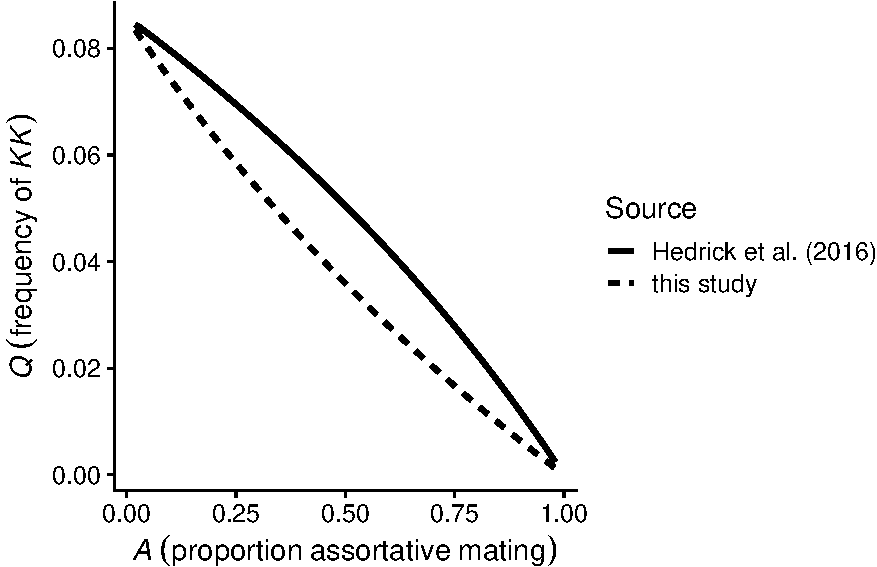
\includegraphics{ms_files/figure-latex/fig1-1} 

}

\caption{The equilibirum frequency of $Q$, the $KK$ homozygote in this study (dashed line) and Hedrick \textit{et al.} (2016) (solid line) for possible values of $A$, the proportion of wolves mating assortatively by color.}\label{fig:fig1}
\end{figure}

In conclusion, the mathematical error in \protect\hyperlink{ref-hedrick_negative-assortative_2016}{Hedrick et al.} (\protect\hyperlink{ref-hedrick_negative-assortative_2016}{2016}) does not undermine their primary conclusion that negative-assortative mating by color may explain the distribution of genotype frequencies at the beta definsin locus in the Yellowstone population of wolves (\emph{Canis lupus}). The derivation here may prove useful to future research on negative-assortative mating.

\hypertarget{literature-cited}{%
\section*{Literature cited}\label{literature-cited}}
\addcontentsline{toc}{section}{Literature cited}

\hypertarget{refs}{}
\begin{CSLReferences}{1}{0}
\leavevmode\hypertarget{ref-hedrick_population_2012}{}%
Hedrick, P. W., and K. Ritland. 2012. Population genetics of the white-phased "{Spirit}" bear of {British} {Columbia}. Evolution 66:305--313.

\leavevmode\hypertarget{ref-hedrick_negative-assortative_2016}{}%
Hedrick, P. W., D. W. Smith, and D. R. Stahler. 2016. Negative-assortative mating for color in wolves. Evolution 70:757--766.

\leavevmode\hypertarget{ref-meurer_sympy:_2017}{}%
Meurer, A., C. P. Smith, M. Paprocki, O. Čertík, S. B. Kirpichev, M. Rocklin, A. Kumar, S. Ivanov, J. K. Moore, S. Singh, T. Rathnayake, S. Vig, B. E. Granger, R. P. Muller, F. Bonazzi, H. Gupta, S. Vats, F. Johansson, F. Pedregosa, M. J. Curry, A. R. Terrel, Š. Roučka, A. Saboo, I. Fernando, S. Kulal, R. Cimrman, and A. Scopatz. 2017. {SymPy}: Symbolic computing in {Python}. PeerJ Computer Science 3:e103.

\leavevmode\hypertarget{ref-r_core_team_r_2021}{}%
R Core Team. 2021. R: {A} {Language} and {Environment} for {Statistical} {Computing}. R Foundation for Statistical Computing, Vienna, Austria.

\leavevmode\hypertarget{ref-ushey_reticulate_2022}{}%
Ushey, K., J. J. Allaire, and Y. Tang. 2022. Reticulate: {Interface} to '{Python}'.

\end{CSLReferences}

\end{document}
